% GEODISC assignment 1 (Seb) — framework manuscript
% Compile: pdflatex manuscript && bibtex is NOT needed (manual thebibliography)
% Run pdflatex twice for cross-references.
\documentclass[11pt]{article}
\usepackage[a4paper,margin=2.1cm]{geometry}
\usepackage[utf8]{inputenc}
\usepackage[round,authoryear]{natbib}
\usepackage{booktabs,amsmath,amssymb,mhchem,graphicx,caption,microtype,setspace,array}
\usepackage{tikz}
\usetikzlibrary{arrows.meta,positioning,fit,backgrounds}
\setstretch{1.0}
\captionsetup{font=small,labelfont=bf}

\title{\vspace{-1.0cm}\textbf{Oxygen, kerogen, and morphology: a framework for separating
preservational from biological signals across the Great Oxidation Event}}
\author{[Author Name]\\
\small\textit{GEODISC -- Geological Discovery programme, [Institution]}}
\date{}

\begin{document}
\maketitle

\begin{abstract}\small
\noindent The Great Oxidation Event (GOE, $\sim$2.4~Ga) marks the first persistent rise of
atmospheric \ce{O2} above $\sim$$10^{-5}$~PAL. Because low oxygen should slow oxidative degradation
of organic matter, the anoxic Archean might be expected to preserve organic fossils particularly
well; yet morphologically diagnostic microfossils are comparatively rare before the GOE and
diversify afterwards. We argue that this paradox dissolves once two preservation modes are
distinguished: \emph{bulk organic-carbon survival} and \emph{morphological fidelity}. Redox
controls not the total preservation potential alone but the \emph{partitioning} between these
modes, via decay pathways and the availability of early-diagenetic mineral templating
(silicification, pyritisation, phosphatisation). The GOE-driven rise in seawater sulfate made
microbially mediated pyritisation newly available even as rising \ce{O2} sped aerobic decay. We
propose a comparative, multiproxy framework---Raman spectroscopy of carbonaceous matter (maturation
and structural order), iron speciation, and quantitative morphological-fidelity scoring on
lithofacies- and maturity-matched cherts before and after the GOE---integrated through a
mechanistic process-graph model and Bayesian data fusion. Four testable predictions can falsify a
purely biological reading of the post-GOE fossil expansion and quantify the preservational
contribution.
\end{abstract}

\noindent\textbf{Keywords:} Great Oxidation Event; taphonomy; kerogen; Raman spectroscopy;
iron speciation; Precambrian microfossils; pyritisation.

%==================================================================
\section{Introduction: an oxygen--preservation paradox}

Before the GOE, atmospheric \ce{O2} was below $\sim$$10^{-5}$~PAL---low enough that mass-independent
sulfur isotope fractionation (S-MIF), which requires an anoxic atmosphere, was continuously
expressed \citep{Pavlov2002,Farquhar2000}. Archean oceans were dominantly anoxic and ferruginous,
with seawater sulfate concentrations $<$200~\textmu M and perhaps as low as a few \textmu M
\citep{Habicht2002,Crowe2014}. Under such conditions, aerobic respiration---the most efficient
organic-matter (OM) degradation pathway---was suppressed, and one might \emph{a priori} expect the
Archean to be a high-fidelity archive of early life.

Yet the morphological microfossil record tells a different story. Putatively biological structures
are reported from $\ge$3.4~Ga cherts \citep{Schopf1993}, but the oldest widely accepted
microfossils remain hotly contested \citep{Brasier2002}, and unambiguously diverse, morphologically
diagnostic assemblages become abundant only after the GOE---most famously the gunflintia of the
$\sim$1.88~Ga Gunflint Formation \citep[reviewed in][]{Javaux2018,Wacey2014}. The intuitive
expectation---that low oxygen should yield \emph{more} and \emph{better} preserved fossils---is
therefore not obviously met.

This paper concerns a single question: \emph{does the post-GOE expansion of the morphological
fossil record reflect biological diversification, or a shift in what redox conditions allowed to
be preserved?} We do not claim these are mutually exclusive. Instead, we propose a framework to
\emph{partition} the observed signal and, where possible, to falsify a purely biological
explanation. The central working hypothesis is that \emph{preservation of organic carbon and
preservation of morphology are decoupled, and that redox controls their relative availability}
(Fig.~\ref{fig:graph}). This reframes the problem from ``how much biomass was preserved?'' to
``what was preservable, and under which regime?''

%==================================================================
\section{Background}

\subsection{The GOE and the redox landscape}

The GOE---the first persistent rise of atmospheric \ce{O2} above $\sim$$10^{-5}$~PAL
\citep{Holland2002,Holland2006,Canfield2005,Catling2005}---is pinned to $\sim$2.32--2.45~Ga by the
disappearance of mass-independent sulfur isotope fractionation (S-MIF)
\citep{Bekker2004,Farquhar2003}, though the transition was prolonged and oscillatory
\citep{Lyons2014,Garduno2024}. Proposed drivers include organic-carbon burial during the
Lomagundi--Jatuli excursion \citep{Bekker2012,Hodgskiss2023}, hydrogen escape to space
\citep{Catling2001}, a shift to subaerial volcanism that weakened the volcanic \ce{O2} sink
\citep{Kump2007}. Transient pre-GOE ``whiffs'' of
oxygen are reported but contested \citep{Anbar2007,Gregory2022}. Mid-Proterozoic \ce{O2} remained
at $\sim$1--10\%~PAL \citep{Lyons2014} or as low as $\le$0.1\%~PAL \citep{Planavsky2014}, and the
deep ocean stayed largely anoxic---ferruginous with euxinic wedges
\citep{Canfield1998}. Critically for what follows, seawater sulfate rose across the
GOE from trace (\textmu M) levels to millimolar levels \citep{Habicht2002,Kah2004,Crowe2014}. Local
redox is reconstructed from iron speciation
\citep[$\mathrm{Fe_{HR}}/\mathrm{Fe_T}>0.38$;][]{Poulton2005,Poulton2011}, chromium isotopes
\citep{Frei2009}, and Mo--U--N systematics \citep{Scott2008,Garvin2009}. The proxies
together document a transition in which the \emph{character} of anoxia changed as much as its
spatial extent.

\subsection{The Precambrian microfossil record}

The Archean microfossil record is sparse and contentious: the filamentous structures of the
$\sim$3.46~Ga Apex chert \citep{Schopf1993} were reinterpreted as abiogenic mineral artefacts
\citep{Brasier2002}, and even better-preserved Archean microbiotas (Strelley Pool, $\sim$3.4~Ga;
Tumbiana, $\sim$2.7~Ga) are typically mat-related and morphologically simple. After the GOE the
record becomes qualitatively richer, with Gunflint-type assemblages (filaments, coccoids,
spindle-shaped forms) widespread in $\sim$1.9~Ga shallow-marine cherts and taxonomically
resolvable \citep{Javaux2018,Wacey2012,Wacey2014}. The transition from ``mats and kerogen'' to
``diagnostic microfossils'' across the GOE is the empirical phenomenon we seek to explain.

\subsection{Two modes of preservation}

\emph{Organic-carbon survival}---whether biomass escapes remineralisation and is buried as
kerogen---is governed by oxygen-exposure time, sedimentation rate, the intrinsic recalcitrance of
biomolecules, and mineral (especially iron-) surface protection
\citep{Canfield1994,Hedges1995,Hartnett1998,Lalonde2012}. Anoxia aids OM survival by suppressing
aerobic respiration, and $\sim$20\% of sedimentary organic carbon is directly bound to reactive
iron phases \citep{Lalonde2012}. \emph{Morphological fidelity}, by contrast, is won or lost in a
race between decay and early-diagenetic mineral templating: cellular structure is preserved only
when silica, pyrite, phosphate or clay minerals impregnate or encrust cells \emph{before} decay
collapses morphology \citep{Wacey2012}. These two modes share decay as a common antagonist but
depend on different---and independently variable---mineral pathways. Anoxia therefore favours OM
survival unambiguously, but its effect on morphological fidelity is conditional on whether the
requisite mineral-templating pathway is available.

\subsection{Raman spectroscopy of carbonaceous matter}

Raman spectroscopy of carbonaceous material (CM) provides two complementary constraints.
Peak-metamorphism thermometry, calibrated by \citet{Beyssac2002}, relates the relative area of the
defect (D1) and graphite (G) bands---commonly expressed as
\begin{equation}
R_2 = \frac{A_{D1}}{A_{D1}+A_{G1}+A_{G2}}
\end{equation}
to maximum temperature, allowing samples to be matched for thermal maturity. The D--G parameters
and their spatial heterogeneity also report the \emph{structural order} (aromaticity /
carbonisation) of the CM \citep{Qu2019}, so that differences in preservation pathway can leave a
signature in CM structure beyond the temperature record. Raman mapping thus lets us compare both
thermal history and CM structural character across the GOE on a common basis.

%==================================================================
\section{Hypothesis: a redox-modulated preservation regime}

We propose that the GOE did not simply raise or lower ``preservation'' but shifted the
\emph{preservation regime}---the mapping from environmental redox onto the two preservation
modes---because the availability of the decisive mineral-templating pathways is itself
redox-sensitive in ways that do not track \ce{O2} alone:

\begin{itemize}\itemsep0pt
\item \textbf{Pyritisation requires sulfate.} Microbial sulfate reduction yields \ce{H2S} that
encrusts and replaces cells; this pathway was muted in the sulfate-starved Archean ocean
\citep{Habicht2002,Crowe2014} and activated only after the GOE \citep{Kah2004}, making a
high-fidelity preservation mode newly available even as rising \ce{O2} sped aerobic decay.
\item \textbf{Silicification depends on the silica cycle, not directly on \ce{O2}.} Archean oceans
were silica-rich in the absence of biological silica sinkers, so silicification potential was
arguably \emph{high} before the GOE---yet Archean silicified assemblages are not correspondingly
morphologically rich, suggesting decay commonly outpaced mineralisation, or that mat texture rather
than cellular fidelity was preferentially captured.
\item \textbf{Decay community tracks electron acceptors.} The dominant OM-oxidation pathway shifts
with redox (aerobic respiration $\to$ sulfate reduction $\to$ methanogenesis), changing both the
\emph{rate} and the \emph{selectivity} of decay, and hence which morphological characters survive.
\end{itemize}

\begin{figure}[t]
\centering
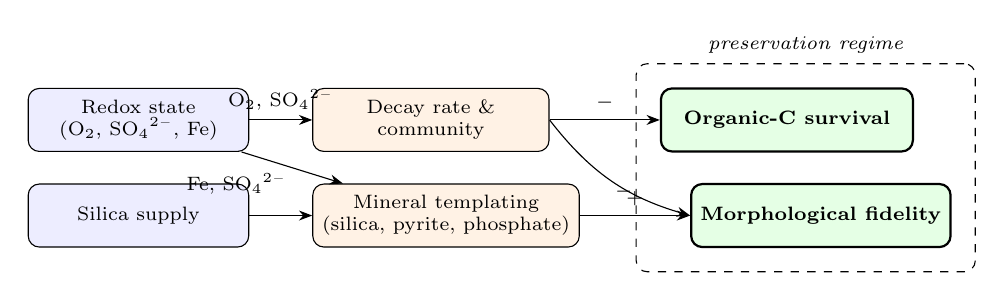
\begin{tikzpicture}[
  >=Stealth, node distance=4mm and 8mm,
  drv/.style={draw,rounded corners,align=center,fill=blue!7,minimum width=28mm,minimum height=8mm,font=\scriptsize},
  prc/.style={draw,rounded corners,align=center,fill=orange!10,minimum width=30mm,minimum height=8mm,font=\scriptsize},
  outp/.style={draw,thick,rounded corners,align=center,fill=green!10,minimum width=32mm,minimum height=8mm,font=\scriptsize},
  every node/.style={font=\scriptsize}]
\node[drv] (redox) {Redox state\\(\ce{O2}, \ce{SO4^{2-}}, Fe)};
\node[drv,below=of redox] (silica) {Silica supply};
\node[prc,right=of redox] (decay) {Decay rate \&\\community};
\node[prc,right=of silica] (miner) {Mineral templating\\(silica, pyrite, phosphate)};
\node[outp,right=14mm of decay] (om) {\textbf{Organic-C survival}};
\node[outp,right=14mm of miner] (morph) {\textbf{Morphological fidelity}};
\draw[->] (redox) -- node[above,font=\scriptsize]{\ce{O2}, \ce{SO4^{2-}}} (decay);
\draw[->] (redox) -- node[below left=-2pt,font=\scriptsize]{Fe, \ce{SO4^{2-}}} (miner);
\draw[->] (silica) -- (miner);
\draw[->] (decay) -- node[above,font=\scriptsize]{$-$} (om);
\draw[->] (decay.east) to[bend right=18] node[below right=-3pt,font=\scriptsize]{$-$} (morph.west);
\draw[->] (miner) -- node[above,font=\scriptsize]{$+$} (morph);
\begin{scope}[on background layer]
\node[draw,dashed,rounded corners,fit=(om)(morph),inner sep=3mm,label={[font=\scriptsize\itshape]above:preservation regime}] {};
\end{scope}
\end{tikzpicture}
\caption{Mechanistic preservation process graph. Redox and silica supply (left) set the decay rate
and the availability of mineral-templating pathways (centre), which independently control the two
preservation outputs (right). Because mineral-templating availability depends on sulfate and iron,
not on \ce{O2} alone, the two outputs can vary independently across the GOE. The graph is the
quantitative model fit during data fusion (Sec.~\ref{sec:frame}).}
\label{fig:graph}
\end{figure}

This yields a clear, non-trivial expectation: across the GOE, \emph{morphological fidelity} should
rise (as pyritisation and other post-GOE pathways activate) even where \emph{bulk OM survival} does
not, and possibly where anoxia-driven OM survival declines. The post-GOE ``more fossils'' signal
need not imply more biomass.

%==================================================================
\section{Proposed framework}\label{sec:frame}

\subsection{Sample and archival strategy}

The central experimental challenge is to isolate redox from confounders---thermal maturity,
lithofacies, and rock volume. We therefore propose paired comparison of shallow-marine
silicified carbonates and cherts deposited before and after the GOE, matched as closely as possible
on lithofacies and on Raman peak maturity ($R_2$/Tmax), and normalised per unit host rock. Candidate
units span the boundary (Table~\ref{tab:forms}). Existing museum collections, drilled cores, and
published Raman/kerogen datasets provide immediate material without new fieldwork; a targeted
sampling campaign of two or three pre-/post-GOE pairs would anchor new analyses.

\begin{table}[t]
\centering\small
\caption{Candidate units for a lithofacies- and maturity-matched pre/post-GOE comparison. All are
shallow-marine, silicified, and low metamorphic grade.}
\label{tab:forms}
\begin{tabular}{lllll}
\toprule
Formation & Age (Ga) & Lithology & Setting & Relative to GOE \\
\midrule
Strelley Pool & $\sim$3.4 & chert/carb. & shallow mar., stromatolitic & pre \\
Tumbiana Gp. & $\sim$2.7 & strom. carb./chert & lacustrine--marg. marine & pre \\
Belingwe (Ngarangan) & $\sim$2.7 & strom. carb. & shallow marine & pre \\
\midrule
Belcher Gp. & $\sim$2.0 & chert/dolostone & shallow marine & post \\
Gunflint Fm. & $\sim$1.88 & chert & shallow mar., foreshore & post \\
Sokoman IF & $\sim$1.88 & cherty carb./oxide & shelf & post \\
\bottomrule
\end{tabular}
\end{table}

\subsection{Analytical programme}

On each matched sample we propose five measurements:
\begin{enumerate}\itemsep0pt
\item \textbf{Raman CM mapping} ($R_2$ for maturity control; D--G band ratios and spatial
heterogeneity for structural order / aromaticity), following the metrology of \citet{Beyssac2002}
and the microfossil-application practice of \citet{Qu2019}.
\item \textbf{Iron speciation} \citep{Poulton2005} and pyrite iron, to reconstruct local redox and
quantify the pyritisation flux.
\item \textbf{Total organic carbon} (TOC) and, where possible, CM major-element H/C as an
independent maturity/aromaticity index.
\item \textbf{Morphological-fidelity scoring} of associated microfossils, performed blind to age
and redox, on a defined ordinal scale (cell-wall integrity, internal detail, taxonomic
discriminability), with multiple scorers and inter-rater reliability metrics.
\item \textbf{Ancillary redox/nutrient proxies} on a subset: sulfur isotopes, Mo--U enrichments
\citep{Scott2008}, and $\delta^{15}$N \citep{Garvin2009}.
\end{enumerate}

\subsection{Data synthesis, experiments, and integration}

We compile published Raman/kerogen, iron-speciation, and microfossil-quality data across the GOE
into a unified database, testing---by rarefaction and per-unit-rock normalisation---whether the
apparent post-GOE richness survives correction for sampled rock volume. In parallel, laboratory
decay--mineralisation experiments on cyanobacterial/mat analogues, factorial in
\ce{O2}~$\times$~sulfate~$\times$~reactive Fe, would directly measure OM survival against
morphological fidelity under each regime, orthogonalising the redox variables that co-varied
across the GOE. Finally, the preservation outputs and their drivers (Fig.~\ref{fig:graph}) form a
causal graph whose edges carry probabilities and uncertainties: rather than regress ``fossil
abundance'' on environment, we treat the partition as Bayesian inversion over hidden processes
(decay regime, pyritisation flux, silicification rate), comparing preservational-shift,
biological-expansion, and combined models by marginal likelihood. The graph makes the load-bearing
assumption---that decay opposes both outputs while mineral templating supports only
morphology---explicit and falsifiable.

\subsection{Ruling out alternatives}

Four non-redox explanations must be explicitly addressed:
(i) \emph{metamorphic overprint}---controlled by matching on $R_2$/Tmax;
(ii) \emph{sampling/rock-volume bias}---addressed by rarefaction and per-volume normalisation;
(iii) \emph{true biological expansion}---predicted by the appearance of genuinely novel
morphotypes that co-occur with better mineralisation only if expansion is real; and
(iv) \emph{facies mismatch}---controlled by lithofacies matching (Table~\ref{tab:forms}).

%==================================================================
\section{Testable predictions}

\begin{table}[t]
\centering\small
\caption{Predictions of the preservational-shift hypothesis and the observations that would
distinguish it from a purely biological expansion.}
\label{tab:preds}
\begin{tabular}{p{0.32\linewidth}p{0.30\linewidth}p{0.30\linewidth}}
\toprule
Prediction & Supports preservational shift & Supports biology \\
\midrule
P1. Pre-GOE samples, maturity-matched, are OM-rich but morphology-poor, with low pyrite-Fe & high TOC + low fidelity + low \ce{Fe_{pyrite}} & --- \\
P2. Morphology correlates with mineral-templating proxies, not with TOC/anoxia alone & fidelity $\sim$ \ce{Fe_{pyrite}} + silica texture & fidelity $\sim$ TOC \\
P3. The fidelity--OM slope changes across the GOE (interaction term) & significant age$\times$OM interaction & no interaction \\
P4. In decay experiments, oxic/+sulfate treatments preserve morphology best despite lower OM survival & morphology $\uparrow$ while OM $\downarrow$ & morphology tracks OM \\
\bottomrule
\end{tabular}
\end{table}

Under a purely biological expansion, none of P1--P3 should hold: morphology would track OM
abundance, pyrite would not be predictive, and the fidelity--OM relationship would be invariant
across the GOE. The four predictions are thus mutually reinforcing and falsifiable on the proposed
data.

%==================================================================
\section{Implications}

If the preservational-shift hypothesis is supported, the post-GOE ``rise'' of microfossils is
partly a taphonomic artefact of redox-driven mineral-pathway activation---most conspicuously
sulfate-enabled pyritisation---rather than evidence of a contemporaneous biological radiation. The
practical consequences are threefold. First, quantitative estimates of Proterozoic biomass or
diversity that treat fossil abundance as a direct biological signal are biased and should be
redox-corrected. Second, the timing of genuine biological innovations (e.g.\ the origin of
oxygenic photosynthesis, eukaryotes) must be inferred from preservational proxies, not from first
appearances alone. Third, the same logic applies to the search for biosignatures on Mars and in
other Archean-analogue settings: the absence of morphological fossils in an anoxic succession does
not entail the absence of life, only the absence of the mineral pathway required to record it.

%==================================================================
\section{Conclusions}

We have argued that the apparent paradox of an Archean that is organic-rich yet morphology-poor is
resolved by separating two preservation modes that redox affects differently. The GOE's most
consequential taphonomic legacy may be the activation of sulfate-driven pyritisation, which
preserved morphology even as oxidising conditions nominally hastened decay. We propose a
multiproxy, lithofacies- and maturity-matched comparison of pre- and post-GOE cherts---Raman CM,
iron speciation, quantitative morphology---embedded in a mechanistic process-graph model with
Bayesian data fusion, and we give four falsifiable predictions. The framework is designed so that
a purely biological account of the post-GOE fossil expansion can be tested, and---if it fails---so
that the preservational contribution can be quantified rather than merely asserted.

%==================================================================
\bibliographystyle{plainnat}
\begin{thebibliography}{99}\footnotesize\linespread{0.92}\selectfont\setlength{\itemsep}{0pt}\setlength{\parskip}{0pt}
\bibitem[Anbar et al.(2007)]{Anbar2007} Anbar, A.~D., et al. (2007). A whiff of oxygen before the
Great Oxidation Event? \textit{Science}, 317, 1903--1906.
\bibitem[Bekker et al.(2004)]{Bekker2004} Bekker, A., et al. (2004). Dating the rise of atmospheric
oxygen. \textit{Nature}, 427, 117--120.
\bibitem[Bekker \& Holland(2012)]{Bekker2012} Bekker, A., \& Holland, H.~D. (2012). Oxygen overshoot
and recovery during the early Paleoproterozoic. \textit{Earth and Planetary Science Letters},
317--318, 295--304.
\bibitem[Beyssac et al.(2002)]{Beyssac2002} Beyssac, O., Goff\'{e}, B., Chopin, C., \& Rouzaud,
J.~N. (2002). Raman spectra of carbonaceous material in metasediments: a new geothermometer.
\textit{Journal of Metamorphic Geology}, 20, 859--871.
\bibitem[Brasier et al.(2002)]{Brasier2002} Brasier, M.~D., et al. (2002). Questioning the evidence
for Earth's oldest fossils. \textit{Nature}, 416, 76--81.
\bibitem[Canfield(1994)]{Canfield1994} Canfield, D.~E. (1994). Factors influencing organic carbon
preservation in marine sediments. \textit{Chemical Geology}, 114, 315--329.
\bibitem[Canfield(1998)]{Canfield1998} Canfield, D.~E. (1998). A new model for Proterozoic ocean
chemistry. \textit{Nature}, 396, 450--453.
\bibitem[Canfield(2005)]{Canfield2005} Canfield, D.~E. (2005). The early history of atmospheric
oxygen: homage to Robert M.~Garrels. \textit{Annual Review of Earth and Planetary Sciences}, 33,
1--36.
\bibitem[Catling \& Claire(2005)]{Catling2005} Catling, D.~C., \& Claire, M.~W. (2005). How Earth's
atmosphere evolved to an oxic state: a status report. \textit{Earth and Planetary Science Letters},
237, 1--20.
\bibitem[Catling et al.(2001)]{Catling2001} Catling, D.~C., Zahnle, K.~J., \& McKay, C.~P. (2001).
Biogenic methane, hydrogen escape, and the irreversible oxidation of early Earth. \textit{Science},
293, 839--843.
\bibitem[Crowe et al.(2014)]{Crowe2014} Crowe, S.~A., et al. (2014). Sulfate was a trace constituent
of the Archean ocean. \textit{Science}, 346, 735--739.
\bibitem[Farquhar et al.(2000)]{Farquhar2000} Farquhar, J., Bao, H., \& Thiemens, M. (2000).
Atmospheric influence of Earth's earliest sulfur cycle. \textit{Science}, 289, 756--758.
\bibitem[Farquhar \& Wing(2003)]{Farquhar2003} Farquhar, J., \& Wing, B.~A. (2003). Multiple sulfur
isotopes and the evolution of the atmosphere. \textit{Earth and Planetary Science Letters}, 213,
1--13.
\bibitem[Frei et al.(2009)]{Frei2009} Frei, R., Gaucher, C., Poulton, S.~W., \& Canfield, D.~E.
(2009). Fluctuations in Precambrian atmospheric oxygenation recorded by chromium isotopes.
\textit{Nature}, 461, 250--253.
\bibitem[Gardu\~{n}o Ruiz et al.(2024)]{Garduno2024} Gardu\~{n}o Ruiz, D., Goldblatt, C., \& Ahm,
A.-S.~C. (2024). Climate variability leads to multiple oxygenation episodes across the Great
Oxidation Event. \textit{Geophysical Research Letters}, 51, e2023GL106694.
\bibitem[Garvin et al.(2009)]{Garvin2009} Garvin, J., Buick, R., Anbar, A.~D., Arnold, G.~L., \&
Kaufman, A.~J. (2009). Isotopic evidence for an aerobic nitrogen cycle in the latest Archean.
\textit{Science}, 323, 1045--1048.
\bibitem[Gregory et al.(2022)]{Gregory2022} Gregory, D.~D., et al. (2022). Reexamination of
2.5-Ga ``whiff'' of oxygen interval points to anoxic ocean before the Great Oxidation Event.
\textit{Science Advances}, 8, eabj7190.
\bibitem[Habicht et al.(2002)]{Habicht2002} Habicht, K.~S., Gade, M., Thamdrup, B., Berg, P., \&
Canfield, D.~E. (2002). Calibration of sulfate levels in the Archean ocean. \textit{Science}, 298,
2372--2374.
\bibitem[Hartnett et al.(1998)]{Hartnett1998} Hartnett, H.~E., Keil, R.~G., Hedges, J.~I., \& Devol,
A.~H. (1998). Influence of oxygen exposure time on organic carbon preservation in continental
margin sediments. \textit{Nature}, 391, 572--575.
\bibitem[Hedges \& Keil(1995)]{Hedges1995} Hedges, J.~I., \& Keil, R.~G. (1995). Sedimentary organic
matter preservation: an assessment and speculative synthesis. \textit{Marine Chemistry}, 49,
81--115.
\bibitem[Hodgskiss et al.(2023)]{Hodgskiss2023} Hodgskiss, M.~S.~W., Crockford, P.~W., \& Turchyn,
A. (2023). Deconstructing the Lomagundi--Jatuli carbon isotope excursion. \textit{Annual Review of
Earth and Planetary Sciences}, 51, 301--330.
\bibitem[Holland(2002)]{Holland2002} Holland, H.~D. (2002). Volcanic gases, black smokers, and the
Great Oxidation Event. \textit{Geochimica et Cosmochimica Acta}, 66, 3811--3826.
\bibitem[Holland(2006)]{Holland2006} Holland, H.~D. (2006). The oxygenation of the atmosphere and
oceans. \textit{Philosophical Transactions of the Royal Society B}, 361, 903--915.
\bibitem[Javaux et al.(2018)]{Javaux2018} Javaux, E.~J., Lepot, K., \& Knoll, A.~H. (2018). The
Paleoproterozoic fossil record: implications for the evolution of the biosphere and geosphere.
\textit{Earth-Science Reviews}.
\bibitem[Kah et al.(2004)]{Kah2004} Kah, L.~C., Lyons, T.~W., \& Frank, T.~D. (2004). Low marine
sulfate and protracted oxygenation of the Proterozoic biosphere. \textit{Nature}, 431, 834--838.
\bibitem[Kump \& Barley(2007)]{Kump2007} Kump, L.~R., \& Barley, M.~E. (2007). Increased subaerial
volcanism and the rise of atmospheric oxygen 2.5 billion years ago. \textit{Nature}, 448,
1033--1036.
\bibitem[Lalonde et al.(2012)]{Lalonde2012} Lalonde, K., Mucci, A., Ouellet, A., \& G\'{e}linas, Y.
(2012). Preservation of organic matter in sediments promoted by iron. \textit{Nature}, 483,
198--200.
\bibitem[Lyons et al.(2014)]{Lyons2014} Lyons, T.~W., Reinhard, C.~T., \& Planavsky, N.~J. (2014).
The rise of oxygen in Earth's early ocean and atmosphere. \textit{Nature}, 506, 307--315.
\bibitem[Pavlov \& Kasting(2002)]{Pavlov2002} Pavlov, A.~A., \& Kasting, J.~F. (2002).
Mass-independent fractionation of sulfur isotopes in Archean sediments: strong evidence for an
anoxic Archean atmosphere. \textit{Astrobiology}, 2, 27--41.
\bibitem[Planavsky et al.(2014)]{Planavsky2014} Planavsky, N.~J., et al. (2014). Low
mid-Proterozoic atmospheric oxygen levels and the delayed rise of animals. \textit{Science}, 346,
635--638.
\bibitem[Poulton \& Canfield(2005)]{Poulton2005} Poulton, S.~W., \& Canfield, D.~E. (2005).
Development of a sequential extraction procedure for iron: implications for iron partitioning in
continentally derived particulates. \textit{Chemical Geology}, 214, 209--221.
\bibitem[Poulton \& Canfield(2011)]{Poulton2011} Poulton, S.~W., \& Canfield, D.~E. (2011).
Ferruginous conditions: a dominant feature of the ocean through Earth's history. \textit{Elements},
7, 107--112.
\bibitem[Qu et al.(2019)]{Qu2019} Qu, Y., Bower, D.~M., et al. (2019). Raman spectroscopy and
structural heterogeneity of carbonaceous matter in Precambrian microfossils. \textit{Organic
Geochemistry}.
\bibitem[Schopf(1993)]{Schopf1993} Schopf, J.~W. (1993). Microfossils of the Early Archean Apex
chert: new evidence of the antiquity of life. \textit{Science}, 260, 640--646.
\bibitem[Scott et al.(2008)]{Scott2008} Scott, C., et al. (2008). Tracing the stepwise oxygenation
of the Proterozoic ocean. \textit{Nature}, 452, 456--459.
\bibitem[Wacey et al.(2012)]{Wacey2012} Wacey, D., Saunders, M., Brasier, M.~D., \& Kilburn, M.~R.
(2012). Taphonomy of very ancient microfossils from the $\sim$3400~Ma Strelley Pool Formation and
$\sim$1900~Ma Gunflint Formation: new insights using a focused ion beam. \textit{Precambrian
Research}.
\bibitem[Wacey et al.(2014)]{Wacey2014} Wacey, D., et al. (2014). Changing the picture of Earth's
earliest fossils (3.5--1.9~Ga) with new approaches and discoveries. \textit{Proceedings of the
National Academy of Sciences}, 111.

\end{thebibliography}

\end{document}
